\documentclass[a4paper,20pt]{report}
\usepackage[spanish]{babel} 
\usepackage[utf8]{inputenc}
%\graphicspath{ {images/} }


\usepackage{fancyhdr}
\usepackage{hlundef}
\usepackage{informe}
\usepackage{hyperref}



\usepackage[table]{xcolor}

\usepackage{enumerate} % Personalizar enumeraciones

\hypersetup{
    colorlinks=true,
    linkcolor=blue,
    filecolor=magenta,      
    urlcolor=blue,
}
\urlstyle{same}


% USO PERSONALIZADO CARATULA
\title{Estrategia de Copias de Seguridad para una Empresa}
\author{\
Roger Colquehuanca Calcina (2013046539)\\
Christian Poma Machicado (2011041702)\\
Angélica Milla Rondón (2010035944)\\
Kevin Cutipa Chambilla (2010037838)\\
Sergio Pérez Chávez (2013000726)\\
Galindo Maquera Mamani (2012042429)\\
}
\date{2016}

\usepackage{natbib}
\usepackage{graphicx} % figuras
\usepackage{subfigure} % subfiguras


\begin{document}

%\pagenumbering{roman} % Paginacion en i, ii, iii,...
\maketitle

\doublespacing

\tableofcontents %Inserta el indice general
%\addcontentsline{toc}{chapter}{CONTENIDO} % INdice en el indice

\listoftables %Inserta el indice de cuadros
\listoffigures %Inserta el indice de figuras

%%% En esta parte se incluye los archivos del informe
\chapter*{INTRODUCCI\'ON}
    \addcontentsline{toc}{chapter}{INTRODUCCI\'ON}

Describir como mínimo 20 líneas una introducción del trabajo a desarrollar
\pagenumbering{arabic} % pagionacion en 1,2,3...


\chapter{OBJETIVOS}

\section{General}
\begin{enumerate}
\item Desarrollar una Guía Técnica de estrategia de copias de Seguridad y Recuperación de Bases de Datos
\end{enumerate}

\section{Espec\'ificos}
\begin{enumerate}
\item Definir qué tipo de backup aplicar y en qué consiste cada uno.
\item Explicar el impacto de las estrategias de backups en las necesidades del espacio.

\end{enumerate}
\chapter{MARCO TEÓRICO}
\section{COPIAS DE SEGURIDAD Y RESTAURACIÓN DE BASES DE DATOS}
Una copia de los datos que se puede utilizar para restaurar y recuperar los datos se denomina copia de seguridad. Las copias de seguridad le permiten restaurar los datos después de un error. Con las copias de seguridad correctas, puede recuperarse de multitud de errores, por ejemplo:



\begin{itemize}
\item       Errores de medios.
\item       Errores de usuario, por ejemplo, quitar una tabla por error.
\item       Errores de hardware, por ejemplo, una unidad de disco dañada o la pérdida permanente de un servidor.
\item       Desastres naturales.
\end{itemize}

 Además, las copias de seguridad de una base de datos son útiles para fines administrativos habituales, como copiar una base de datos de un servidor a otro, configurar la creación de reflejo de la base de datos y el archivo, etc.

\section{CÓMO IMPEDIR LA PÉRDIDA DE LOS DATOS}
Impedir la pérdida de datos es uno de los problemas más importantes que afrontan los administradores de sistemas.

\subsection{Disponer de una estrategia de copia de seguridad}
Debe tener una estrategia de copia de seguridad para aminorar la pérdida de datos y recuperar los datos perdidos. Los datos se pueden perder como consecuencia de errores de hardware o de software, o bien por:

\begin{itemize}
\item El uso accidental o malintencionado de una instrucción DELETE.
\item  El uso accidental o malintencionado de una instrucción UPDATE; por ejemplo, no utilizar la cláusula WHERE con una instrucción UPDATE (se actualizan todas las filas en lugar de una fila concreta de la tabla).
\item  Virus destructivos.
\item  Desastres naturales, como incendios, inundaciones y terremotos.
\item  Robo.
\end{itemize}

Si utiliza una estrategia de copia de seguridad adecuada, puede restaurar los datos con un costo mínimo sobre la producción y reducir la posibilidad de que los datos se pierdan definitivamente. Piense en la estrategia de copia de seguridad como un seguro. Su estrategia de copia de seguridad debe devolver el sistema al punto en el que se encontraba antes del problema. Al igual que con una póliza de seguros, pregúntese: “¿cuánto estoy dispuesto a pagar y cuántas pérdidas puedo permitirme?”.

Los costos asociados con la estrategia de copia de seguridad incluyen la cantidad de tiempo que se emplea en diseñar, implementar, automatizar y probar los procedimientos de copia de seguridad. Aunque la pérdida de datos no se puede impedir completamente, debe diseñar una estrategia de copia de seguridad para reducir el alcance de los daños. Cuando diseñe una estrategia de copia de seguridad, considere la cantidad de tiempo que se puede permitir que el sistema esté parado, así como la cantidad de datos que se puede admitir perder (si puede perderse alguno) en el caso de un error del sistema.

    
\subsection{Hacer copias de seguridad con regularidad}  
La frecuencia con que haga las copias de seguridad de la base de datos depende de la cantidad de datos que esté dispuesto a perder y la actividad de la base de datos. Cuando haga copias de seguridad de bases de datos de usuario, tenga en cuenta los siguientes hechos e instrucciones:





\begin{itemize}
\item 
 Puede hacer copias de seguridad de la base de datos con frecuencia si el sistema se encuentra en un entorno de proceso de transacciones en línea (OLTP, Online Transaction Processing).

\item 
Puede hacer copias de seguridad de la base de datos con menos frecuencia si el sistema tiene poca actividad o se utiliza, principalmente, para la toma de decisiones.

\item 
Debe programar las copias de seguridad cuando no se estén efectuando muchas actualizaciones en SQL Server.
 
\item 
Tras determinar la estrategia de realización de copias de seguridad, puede automatizar el proceso con el Asistente para planes de mantenimiento de bases de datos.
\end{itemize}




\section{Tipos de respaldo que soporta Oracle}
\begin{itemize}
\item
Completo.- Se respalda toda la base de datos.
\item
Incremental.- Debe tener previamente un respaldo completo. Respalda a medida que se realizan cambios.
\item
Diferencial.- Debe tener previamente un respaldo completo. Respalda las diferencias existentes entre un respaldo y otro.
\item
Flashbacks.- Permite de manera rápida volver a un estado anterior de la base de datos.
\end{itemize}


\subsection{Respaldo y Recuperación}


Para determinar cuándo hacer un respaldo, pensar de la siguiente manera: hacer una copia de respaldo justo antes del momento en que regenerar los datos ocasione mayor esfuerzo que hacer el respaldo.
El respaldo y recuperación de datos es la generación de una copia, en un momento determinado, de los datos del sistema, con vistas a su eventual reposición en caso de pérdida

El respaldo y recuperación de información, trata del esfuerzo necesario para asegurar la continuidad del procesamiento de los datos de las base de datos, con la mínima dificultad posible ante una eventual alteración no deseada de los mismos.

\subsection{Respaldos}

Respaldo es la obtención de una copia de los datos en otro medio magnético, de tal modo que a partir de dicha copia es posible restaurar el sistema al momento de haber realizado el respaldo. Por lo tanto, los respaldos deben hacerse con regularidad, con la frecuencia preestablecida y de la manera indicada, a efectos de hacerlos correctamente.

Es fundamental hacer bien los respaldos. De nada sirven respaldos mal hechos (por ejemplo, incompletos). En realidad, es peor disponer de respaldos no confiables que carecer totalmente de ellos. Suele ocurrir que la realización de respaldos es una tarea relegada a un plano secundario, cuando en realidad la continuidad de una aplicación depende de los mismos. Los respaldos son tan importantes como lo es el correcto ingreso de datos.



\subsubsection{A - Procedimiento de Respaldo y Recuperación} 

1.- Aspectos a considerar

Dado que las aplicaciones (sistemas) tienen características inherentes, para cada aplicación
Corresponde un método apropiado de respaldo y recuperación de datos. Preferentemente, debe ser establecido por quienes desarrollan la aplicación, que son los que saben cuáles datos es necesario respaldar, la mejor manera de hacerlo, etc. y cómo hacer la correspondiente recuperación. Hay que tener en cuenta las características propias del usuario y cuál es la instalación en que funciona el sistema. Es decir, qué computadora, donde está instalada, etc. Incluye el área física (por ejemplo: ambiente aislado o transitado, acondicionamiento térmico, nivel de ruido, etc.).  

Algunos de los aspectos a considerar se presentan a continuación. La lista no es taxativa y el orden de cada aspecto no es relevante, siendo cada aspecto de propósito limitado en forma individual. Un adecuado método de respaldo/recuperación debe tener en cuenta todos los aspectos en conjunto, como ser: 

\begin{itemize}
\item Plan de Respaldo.
\item Cuáles datos se deben incluir - Tipos de respaldos.
\item Cantidad de copias a realizar - Modalidad de copia.
\item Dónde guardarlas.
\item Quienes los manejan.
\item Verificación del respaldo.
\item Registro.
\item Cuándo hacerlo.
\item El respaldo completo del disco.
\item Soporte físico a utilizar para el respaldo 
\end{itemize}
\\
2 .- Plan de Respaldo  
\\
Los procedimientos de respaldo y recuperación desarrollada deben formar parte de un plan de respaldo y recuperación, el cual debe ser documentado y comunicado a todas las personas involucradas. Dado que, a lo largo del tiempo, varias características que se consideran para desarrollar este plan sufren cambios (software utilizado, soporte,
etc.), el plan debe ser revisado, y de ser necesario modificado de manera periódica. 
\\
El plan debe contener todos los ítems detallados a continuación y cualquier otro que mejore la realización del trabajo o clarifique la tarea. 
\\ \\
3 .- Cuáles datos se deben incluir? 
 \\
Cada aplicación maneja un conjunto muy variado de datos, algunos estáticos, otros dinámicos. Hay datos base, a partir de los cuales se generan datos resultantes (información). Al definir el respaldo, se establece si se copian todos los archivos o parte de ellos. Entra en consideración si la copia incluye los propios programas de la aplicación. La decisión final se tomará sobre la base de la criticidad de los datos y el valor de los mismos.  
\\
\\
4 .- Medios de soporte a utilizar 
\\
 Los medios a utilizar dependerá del tipo de computadora (micro. Mainframe, etc.), cantidad de información a almacenar, tiempo disponible para realizar el respaldo, costos y obviamente de la tecnología disponible al momento. \\
Actualmente se cuenta con una variedad muy amplia de soportes disponibles y a costos muy bajos, sobre todo al nivel de micro computadoras. A nivel mainframe las posibilidades se acotan. Las características principales a considerar de cada opción será la capacidad de almacenamiento, medida en Mg o Gb, y la velocidad de transferencia de datos (cantidad de datos por segundo que es posible grabar), medida en Kb/s. Los soportes magnéticos son los más difundidos; también los hay ópticos.  
\\ \\
Las opciones más comunes son (en orden descendente por capacidad de almacenamiento promedio):  
\begin{itemize}
\item - Discos duros.
\item - Cintas (4mm, 8mm, QIC).
\item - Cartuchos (alta densidad, micro)
\item - C D R O M.
\item - Zip drive.
\item - Tarjetas PCM-CIA.
\item - Diskette 
\end{itemize}
\\
5 .- ¿Cuándo realizarlo? 
\\
Para determinar cuándo se realiza el respaldo debemos conocer los tiempos incurridos en desarrollar la tarea y las ventanas de tiempo disponibles en producción (tiempo disponible para realizar tareas que no afecte a los procesos habituales de procesamiento de datos). Los tiempos incurridos en desarrollar la tarea varían dependiendo del soporte utilizado (a mayor velocidad de transferencia menor tiempo incurrido), el tipo de respaldo utilizado (el full back-up es el que lleva mayor cantidad de tiempo) y la cantidad de datos a respaldar (a mayor cantidad mayor tiempo de respaldo). \\
Generalmente, en las empresas, las ventanas de tiempo disponibles durante las semanas son chicas, por lo que se combinan los tipos de respaldo  dependiendo del día de la semana. Así, el fin de semana se realiza un respaldo global y durante la semana se realizan respaldos incrementales. Existen momentos en los cuales es necesario realizar respaldos extraordinarios, como ser nueva instalación de una aplicación, o migración de bases de datos o traslado del equipamiento. En estas circunstancias deben realizarse un respaldo global, para estar totalmente cubierto. 
\\\\
6 .- Periodicidad 
\\
Cada cuanto realizar los respaldos dependerá de la cantidad de operaciones realizadas y las ventanas de tiempo disponibles. Usualmente, y como recomendable, los mismos deben realizarse Diariamente Por ejemplo, día a día se hacen respaldos incrementales o diferenciales y una vez por semana se hacen respaldos completos parciales y una al mes respaldos completos totales. Siempre estas decisiones dependen del volumen de los datos, del soporte de almacenamiento disponible, de la velocidad del respaldo, de la importancia de los datos, etc. 
\\\\

\subsection{c). Herramientas a utilizar }
\\
Hay varias herramientas posibles para respaldo de datos. Algunas son muy simples y otras son muy sofisticadas. En algunas aplicaciones o DBMS se disponen de programas propios, guiados por menú, para llevar a cabo estas tareas. En otras, se deben utilizar los comandos del Sistema Operativo o programas utilitarios para respaldos. También hay combinación de ambas situaciones: desde el programa de aplicación se invocan los comandos del sistema operativo u otro programa. 
 
Se le dará prioridad a la herramienta “nativa” de cada aplicación o DBMS, pues están especialmente desarrolladas para respaldar de manera adecuada esos datos, pero la decisión podrá ser utilizar un software especial para respaldar, la decisión final la tomará personal experto. 

\subsubsection{- Dónde guardarlos - distancia y accesibilidad}
\\
Muy importante es establecer en qué lugar se deben guardar las copias. Debe ser bajo llave, con un juego cerca de la computadora y otro fuera del edificio. El juego que está cerca debe estar accesible y el otro debe ser de acceso restringido. Los respaldos pueden estar sobre una estantería, al lado de la computadora o bien en una caja fuerte. Según los datos y la aplicación se establecen las condiciones de almacenamiento. 
\\
Tan importante como llevar a cabo los respaldos con regularidad, es el respetar los criterios de almacenamiento. Intervienen consideraciones del medio ambiente (temperatura, humedad, polvo, etc.) como así también las personas que tienen acceso a la computadora.  
Otro aspecto a tener en cuenta es por cuánto tiempo se guardan los respaldos. Es usual que toda la información que no está en línea se encuentre respaldada, contando con toda la historia de las operaciones de la empresa. Sin embargo esto no es obligatorio, si debemos considerar situaciones legales existentes (reglamentaciones que obligan a guardar cierta información por X tiempo) o potenciales (procesos judiciales).

\subsubsection{- ¿Quienes realizan y manejan los  respaldos? } 
\\
Es fundamental definir qué personas son las encargadas de llevar a cabo los respaldos y las recuperaciones. No es necesario que sean las mismas personas que hagan los dos procesos. Inclusive, en ciertas situaciones, por motivos de seguridad, deben ser distintas. Puede haber varios usuarios que operan la misma aplicación. En estos casos, un subconjunto reducido de ellos, deben ser los responsables de las tareas de respaldo y recuperación de datos. La recuperación siempre debería ser llevada a cabo por dos personas, en lugar de una sola, por seguridad.

\subsubsection{- Verificación del respaldo } 
\\
Usualmente, la tarea electrónica-mecánica de grabación, requerida en las copias, se lleva a cabo correctamente. Sin embargo, la única forma de saber que se grabó bien, es volver a leer la copia grabada y verificar que coincida con lo leído originalmente. Esta verificación insume tiempo adicional. 
 
Es mejor realizar la verificación en otra computadora, y de manera periódica. Dependiendo de la cantidad de respaldo y del historial de errores, es posible aplicar muestreo estadístico para realizar las verificaciones. 

\subsubsection{- Registro }
\\
Se recomienda llevar un registro de los respaldos que se realizan, así como también las eventuales recuperaciones. Este registro es una historia de los respaldos y las recuperaciones llevados a cabo, al cual se agrega toda observación relevante sobre la aplicación, como por ejemplo, cambios de versiones. 
 
Se sugiere disponer de un registro, el cual consta de las siguientes columnas: 
\begin{itemize}
\item{Fecha (día/mes/año)}
\item{Identificación de operador (por ejemplo, sus iniciales}
\item{Identificación del juego de respaldo (por ejemplo, por letra) }
\item{Hora de inicio (hora: minuto)}
\item{Hora de finalización (hora: minuto)}
\item{Resultado}
\item{Rúbrica del operador }
\end{itemize}


“Resultado” es cómo finalizó la ejecución: sin observaciones si terminó correctamente, o bien cuáles anomalías (por ejemplo, cinta con error, corte de luz, etc.). Para cada respaldo se completa una línea. Para cambios de versión, etc, se hace la anotación, a renglón seguido, en forma descriptiva y sintética, con fecha. Para la recuperación se indica “RECUPERACIÓN” y se utilizan dos líneas, para identificar a los dos operadores que realizan el proceso.


\subsubsection {-consejos para hacer los respaldos y las recuperaciones }
Siguen a continuación los consejos para hacer bien los respaldos, en la frecuencia y forma que correspondan, y para llevar a cabo satisfactoriamente las recuperaciones, toda vez que sea necesario. Se los presenta en forma de lista para enfatizarlos: 
\begin{itemize}
\item{Disponer del tiempo suficiente}
\item{No distraerse por ningún concepto}
\item{No hacerlo cuando se esté cansado}
\item{Trabajar ordenado}
\item{Disponer de suficiente cantidad de cintas, diskettes, u otros }
\item{soportes correctamente rotulados}
\item{Contar con otra persona para las recuperaciones}
\item{Permanecer junto a la computadora durante la  tarea}
\item{Verificar una vez por año estado correcto de la computadora}
\item{Verificar una vez por año lectura/grabación de los respaldos}
\item{Tener acceso a otra computadora de similares características}
\end{itemize}


\subsubsection{-Instalaciones grandes}
En instalaciones de computación de mediano y gran parte (con computadoras ‘mainframes’, minis y micros), tal como oficinas y empresas estatales, instituciones bancarias, empresas de l00 o más empleados y operarios, etc., deben existir normas y procedimientos preestablecidos, tanto genéricos como específicos de cada sistema. En dichos centros de cómputo, las tareas de respaldo son una operación más de las habituales, que estén incorporadas en las rutinas diarias, mensuales, etc.

\section{Marco Conceptual}
\textbf{\flushleft{ORACLE}}: Oracle es un sistema de gestión de base de datos relacional considerado como uno de los sistemas de bases de datos más completos, destacando su soporte de transacciones, estabilidad, escalabilidad,soporte multiplataforma.

\textbf{\flushleft{RESPALDOS}}: Las copias de seguridad son un proceso que se utiliza para salvar toda la información, es decir, un usuario, quiere guardar toda la información, o parte de la información, de la que dispone en el PC hasta este momento, realizará una copia de seguridad de tal manera, que lo almacenará en algún medio de almacenamiento tecnológicamente disponible hasta el momento como por ejemplo cinta, DVD, BluRay, discos virtuales (proporcionados por Internet) o simplemente en otro disco duro, para posteriormente poder restaurar el sistema si pierde la información.

\textbf{\flushleft{RECUPERACIÓN}}: Es proteger la base de datos contra fallas lógicas o físicas que destruyan los datos en forma total o parcial. Y a su vez estas fallas pueden afectar al correcto almacenamiento de los datos.
RMAN: Es un método preferido para realizar copias de seguridad de manera eficiente y la recuperación de una base de datos Oracle. RMAN optimiza el rendimiento y el consumo de espacio durante la copia de seguridad con compresión de archivos de la multiplexación y de respaldo, y se integra con Oracle Secure Backup y productos de terceros medios de gestión de backup en cinta.

\textbf{\flushleft{Catálogo RMAN}}: El catálogo de RMAN contiene metadata que RMAN utiliza para respaldar y recuperar la base de datos primaria. Aunque este componente no es obligatorio, ya que podemos respaldar utilizando nada más el control file, se diría que es una buena práctica tenerlo en nuestro ambiente de respaldos y recuperación.

\textbf{\flushleft{Archive Log}}: El archive log permite generar respaldos en caliente de la base de datos, aunque se puede generar el respaldo de la base de datos con RMAN cuando la misma está cerrada (en frío).

\textbf{\flushleft{Backup en Frio}}: Los backups en frio implican parar la BD en modo normal y copiar todos los ficheros sobre los que se asienta. Antes de parar la BD hay que parar también todas las aplicaciones que estén trabajando con la BD. Una vez realizada la copia de los ficheros, la BD se puede volver a arrancar.

\textbf{\flushleft{Backup en Caliente}}: El backup en caliente se realiza mientras la BD está abierta y funcionando en modo ARCHIVELOG. Habrá que tener cuidado de realizarlo cuando la carga de la BD sea pequeña.
Este tipo de backup consiste en copiar todos los ficheros correspondientes a un tablespace determinado, los ficheros redo log archivados y los ficheros de control. Esto para cada tablespace de la BD.



\chapter{DESAROLLO}

\section{PROCEDIMIENTOS PARA LA CREACIÓN DE COPIAS:}
\textbf {Primero se instaló la base de datos Oracle: Oracle Database 11g Release 2 (11.2.0.1.0) Standard Edition, Standard Edition One, and Enterprise Edition} para Windows

\url{http://www.oracle.com/technetwork/database/enterprise-edition/downloads/112010-win64soft-094461.html}

\textbf{Segundo} se utilizó el programa   sql developer para windows, esto fue para migrar la base de datos de mysql a oracle.
Si es que se requiera cambiar el puerto \textbf { oracle exec DBMS\_xdb.sethttpport(‘8082’);}
\url{https://www.youtube.com/watch?v=-LJ_370_88g}

Las copias de seguridad o backups pueden ser físicas y lógicas:

-Las físicas se realizan cuando se copian los ficheros que soportan la BD. Entre estos se encuentran los backups del SO, los backups en frío y los backups en caliente.

\subsection{Backups del SO}

Este tipo de backup implica parar la BD en modo normal y esto la hace inaccesible el sistema mientras se lleva a cabo.


\subsection{Backups de la BD en Frio}

Los backups en frio implican parar la BD en modo normal y copiar todos los ficheros sobre los que se asienta. Antes de parar la BD hay que parar también todas las aplicaciones que estén trabajando con la BD. Una vez realizada la copia de los ficheros, la BD se puede volver a arrancar.


\subsection{Backups de la BD en Caliente}

El backup en caliente se realiza mientras la BD está abierta y funcionando en modo ARCHIVELOG. Habrá que tener cuidado de realizarlo cuando la carga de la BD sea pequeña. Este tipo de backup consiste en copiar todos los ficheros correspondientes a un tablespace determinado, los ficheros redo log archivados y los ficheros de control.

-Las lógicas sólo extraen información de las tablas utilizando comandos SQL y utilizando las herramientas export e import.

\subsection{Backups Lógicos con Export/Import}

Estas utilidades permiten al DBA hacer copias de determinados objetos de la BD, así como restaurarlos o moverlos de una BD a otra. Estas herramientas utilizan comandos del SQL para obtener el contenido de los objetos.

\textbf{NOTA: Una vez que se ha planeado una estrategia de backup y se ha probado, conviene automatizarla para facilitar así su cumplimiento.}

\begin{figure}[h]
\centering
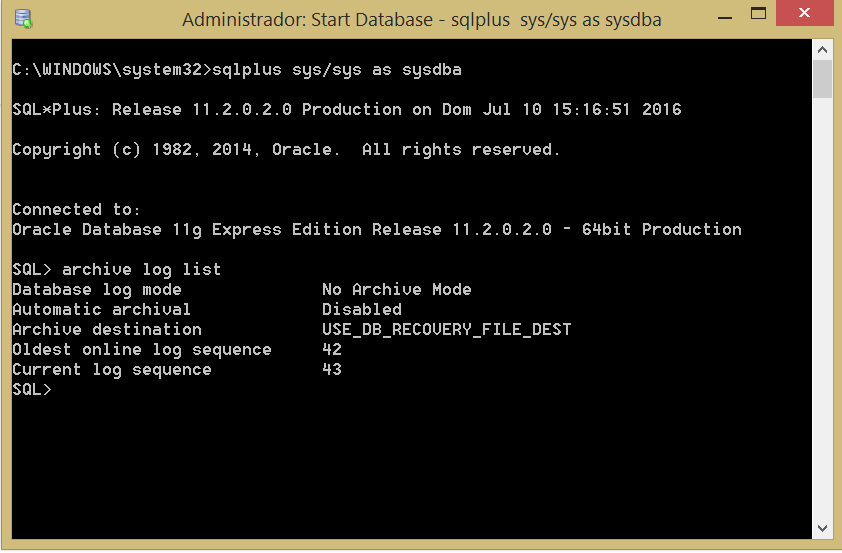
\includegraphics[scale=1.7]{../images/ingresarsqlplus.png}
\caption{Ingresar a sqlplus como sysdba}
\label{fig:ingresar}
\end{figure}

\begin{figure}[h]
\centering
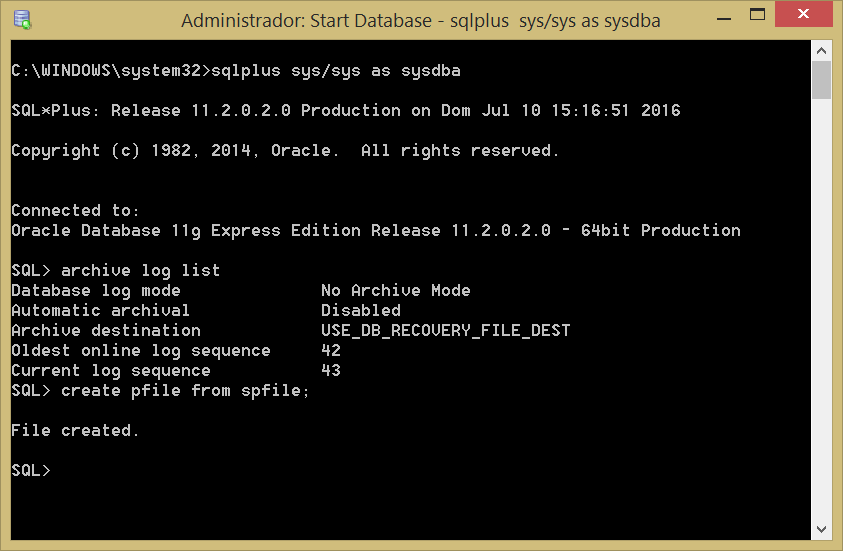
\includegraphics[scale=1.7]{../images/spfile.png}
\caption{Create archivo spfile}
\label{fig:spfile}
\end{figure}

\begin{figure}[h]
\centering
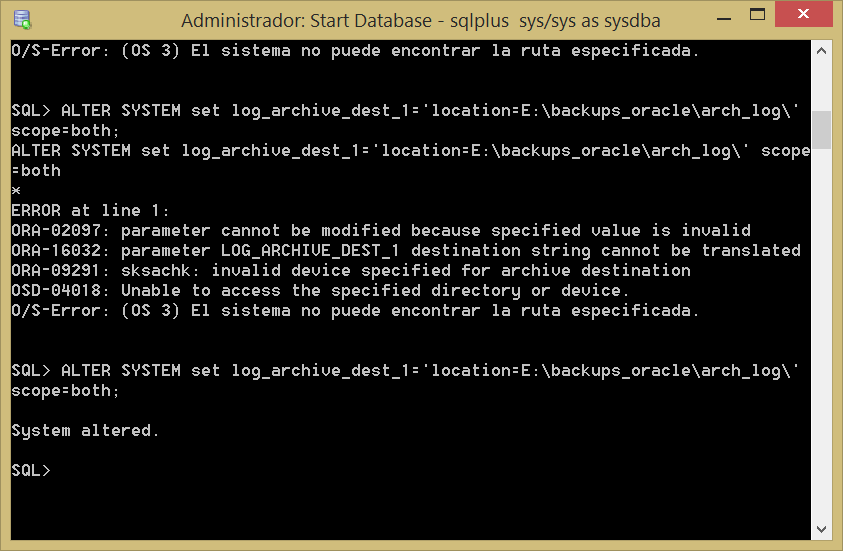
\includegraphics[scale=1.7]{../images/startdb.png}
\caption{Iniciando la Base de Datos}
\label{fig:startdb}
\end{figure}

\begin{figure}[h]
\centering
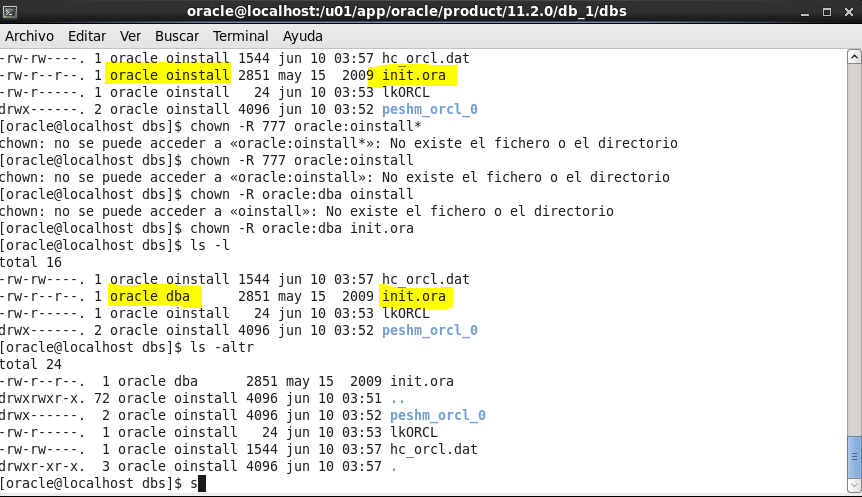
\includegraphics[scale=1.7]{../images/linux.png}
\caption{Iniciando la Base de Datos}
\label{fig:linux}
\end{figure}



\chapter{BACKUPS  DESDE  ENTERPRISE  MANAGER:}\label{cap:1}
\begin{figure}[h]
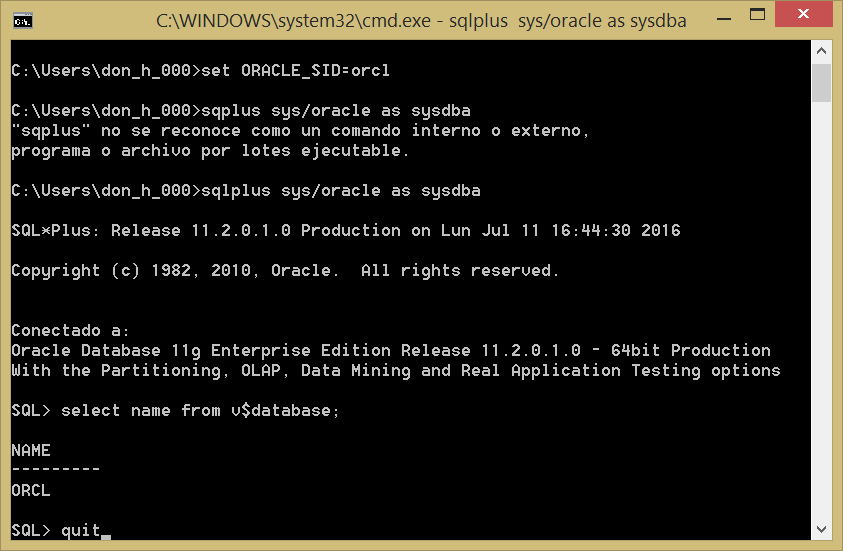
\includegraphics[width=1\textwidth]{../images/backupEM-1.jpg}
\caption{Una  vez  logueados  en  EM,  iremos  al  apartado  “Disponibilidad”  y  apuntaremos  a
“Planificar Copia de Seguridad”.}
\label{fig:bear}
\end{figure}

\begin{figure}[h]
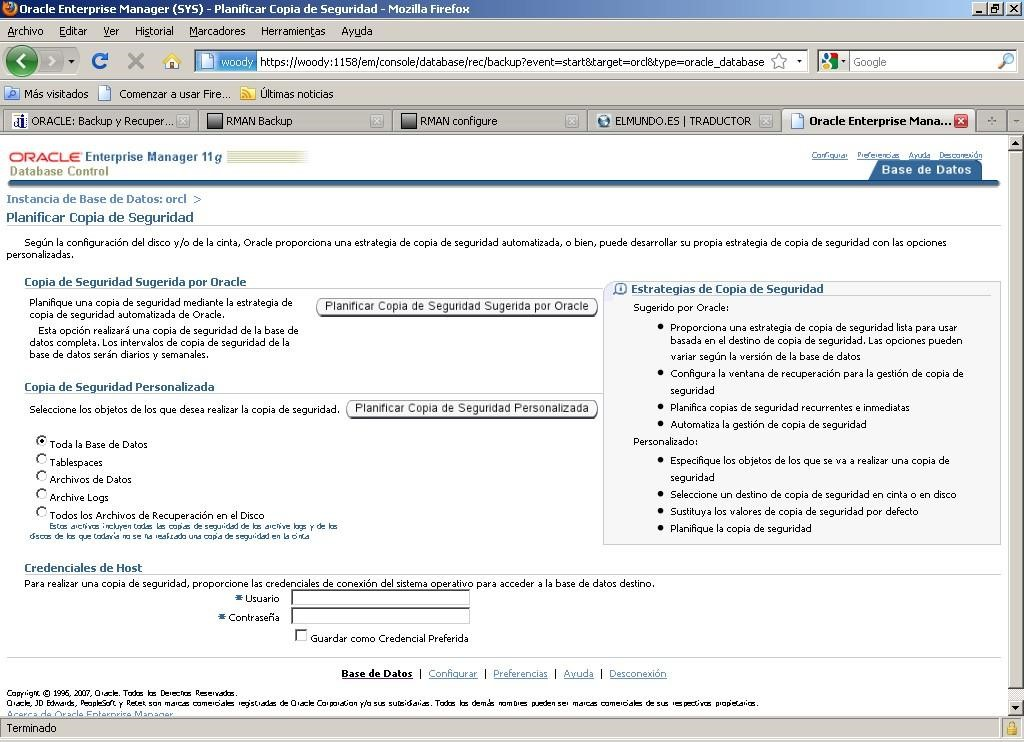
\includegraphics[width=1\textwidth]{../images/backupEM-2.jpg}
\caption{Como vemos nos da 2 opciones a elegir. En este documento analizaremos la opción personalizada con toda la base de datos.
Deberemos conectarnos con los credenciales de host para realizar esta tarea.}
\label{fig:bear}
\end{figure}

\begin{figure}[h]
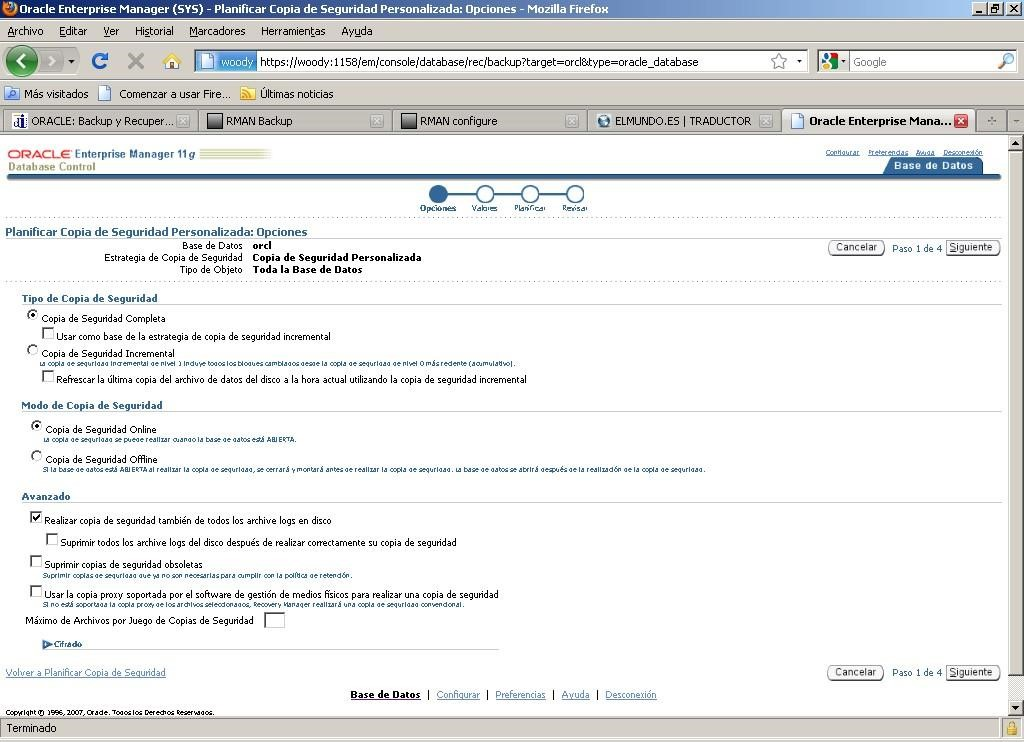
\includegraphics[width=1\textwidth]{../images/backupEM-3.jpg}
\caption{Como  es  la  primera  copia  que  realizamos  deberíamos  elegir  “Copia  de  Seguridad
Completa”.
Para el modo de copia elegiremos si deseamos hacer la copia con la base de datos abierta o cerrada.
En las opciones avanzadas tan sólo añadiremos que realice copia también de los archive logs.}
\label{fig:bear}
\end{figure}

\begin{figure}[h]
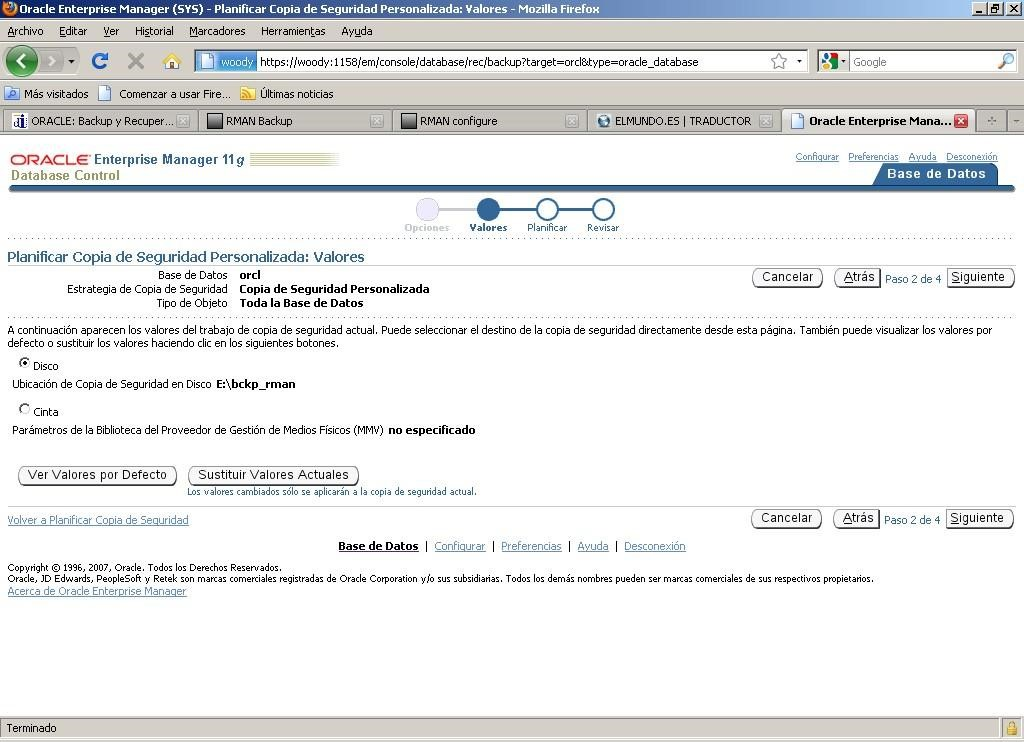
\includegraphics[width=1\textwidth]{../images/backupEM-4.jpg}
\caption{En este paso elegiremos el destino de la copia. Como no dispongo de dispositivo de cintas pasó a continuar explicando la opción “Disco”. (La ubicación que ha tomado para la opción “Disco” esta asignada desde RMAN).}
\label{fig:bear}
\end{figure}

\begin{figure}[h]
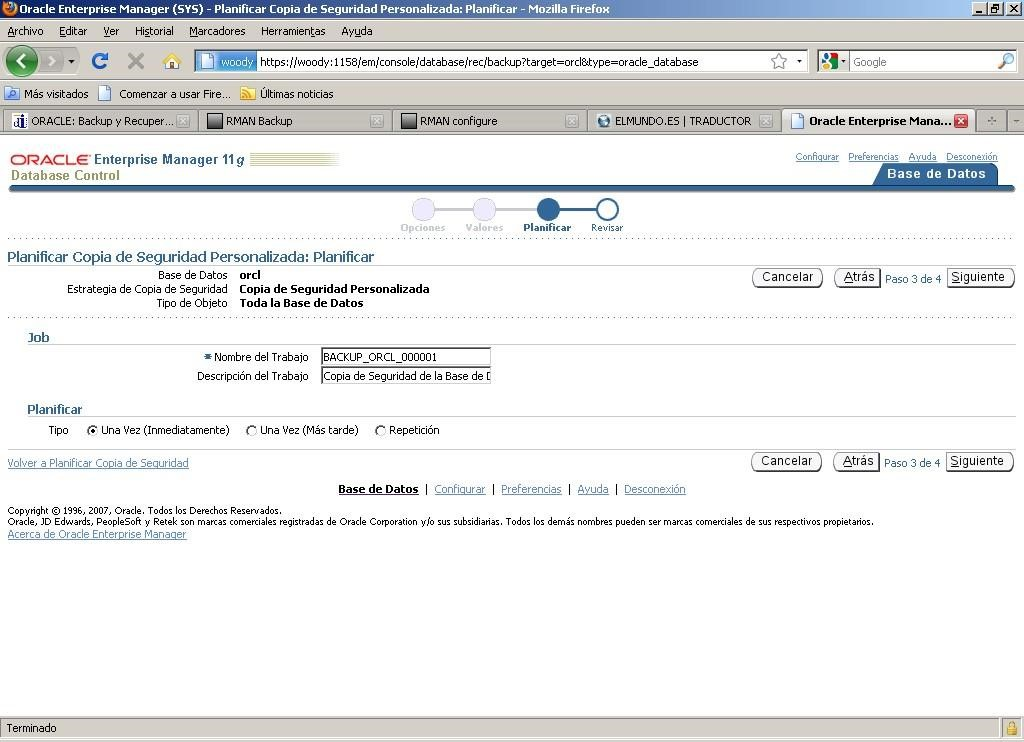
\includegraphics[width=1\textwidth]{../images/backupEM-5.jpg}
\caption{Introducimos nombre si lo deseamos y la descripción, y lo planificamos para que se realice una vez y de forma inmediata.}
\label{fig:bear}
\end{figure}


\chapter{CONCLUSIONES}
    \addcontentsline{toc}{chapter}{CONCLUSIONES}

\begin{enumerate}
\item La planeación de una buena estrategia de backup y de restauración es imprecindible para agilizar la restauracion de información
\item Un Estrategia de backup va a depender los datos a respaldar

\item Se pueden realizar backups con la base de datos conectada o desconectada ademas de por modo consola o grafica con el Enterprise Manager
\end{enumerate}
\chapter*{RECOMENDACIONES}
    \addcontentsline{toc}{chapter}{RECOMENDACIONES}

El estudiante podrá sugerir todas las recomendaciones y observaciones referidas al desarrollo de la práctica. Debiendo explicar las causas, si fuera el caso, de resultados obtenidos distintos a los esperados.

\begin{enumerate}
\item Primera Conclusi\'on
\item Segunda Conclusi\'on
\end{enumerate}
\renewcommand{\bibname}{BIBLIOGRAFIA}
\bibliographystyle{plain}
\bibliography{Bibliografia}

\renewcommand\appendixname{Anexo}
\appendix
\chapter{CODIGO SQL}


\section{Postulado01}

\end{document}